
%(BEGIN_QUESTION)
% Copyright 2006, Tony R. Kuphaldt, released under the Creative Commons Attribution License (v 1.0)
% This means you may do almost anything with this work of mine, so long as you give me proper credit

Determine a basic 5-point (0\%, 25\%, 50\%, 75\%, and 100\%) calibration table for the displacer level transmitter in this scenario:

$$\includegraphics[width=15.5cm]{i00688x01.eps}$$

The cylindrical displacer weighs 8 pounds (dry) and has a diameter of 2.5 inches.  The process liquid is at a temperature of 52 degrees F and has a density of 60 lb/ft$^{3}$.  The 0\% process liquid level (LRV) is even with the bottom of the displacer.  Assume an electronic transmitter mechanism with an output range of 4 to 20 mA, and a calibration tolerance of $\pm$ 0.2\% (of span).

% No blank lines allowed between lines of an \halign structure!
% I use comments (%) instead, so that TeX doesn't choke.

$$\vbox{\offinterlineskip
\halign{\strut
\vrule \quad\hfil # \ \hfil & 
\vrule \quad\hfil # \ \hfil & 
\vrule \quad\hfil # \ \hfil & 
\vrule \quad\hfil # \ \hfil & 
\vrule \quad\hfil # \ \hfil & 
\vrule \quad\hfil # \ \hfil \vrule \cr
\noalign{\hrule}
%
% First row
Process & Percent of & Buoyant & Output signal & Output signal & Output signal \cr
%
% Another row
level (in) & span (\%) & force (lb) & ideal (mA) & min. (mA) & max. (mA) \cr
%
\noalign{\hrule}
%
% Another row
  & 0 &  &  &  &  \cr
%
\noalign{\hrule}
%
% Another row
  & 25 &  &  &  &  \cr
%
\noalign{\hrule}
%
% Another row
  & 50 &  &  &  &  \cr
%
\noalign{\hrule}
%
% Another row
  & 75 &  &  &  &  \cr
%
\noalign{\hrule}
%
% Another row
  & 100 &  &  &  &  \cr
%
\noalign{\hrule}
} % End of \halign 
}$$ % End of \vbox

\vskip 10pt

Be sure to show all your mathematical work so that your instructor will be able to check the conceptual validity of your technique(s).  A good way to check to see if you're solving the problem correctly is to check that each and every one of your intermediate calculations (i.e. the results you get mid-way during the process to arrive at the final answer) has real physical meaning.  {\bf If you truly understand what you are doing, you will be able to identify the correct unit of measurement for every intermediate result and also be able to show where that number applies to the scenario at hand}.


\vskip 20pt \vbox{\hrule \hbox{\strut \vrule{} {\bf Suggestions for Socratic discussion} \vrule} \hrule}

\begin{itemize}
\item{} Demonstrate how to {\it estimate} numerical answers for this problem without using a calculator.
\item{} Calculate the apparent weight of the displacer in each of these process level conditions.
\end{itemize}

\underbar{file i00688}
%(END_QUESTION)





%(BEGIN_ANSWER)

% No blank lines allowed between lines of an \halign structure!
% I use comments (%) instead, so that TeX doesn't choke.

$$\vbox{\offinterlineskip
\halign{\strut
\vrule \quad\hfil # \ \hfil & 
\vrule \quad\hfil # \ \hfil & 
\vrule \quad\hfil # \ \hfil & 
\vrule \quad\hfil # \ \hfil & 
\vrule \quad\hfil # \ \hfil & 
\vrule \quad\hfil # \ \hfil \vrule \cr
\noalign{\hrule}
%
% First row
Process & Percent of & Buoyant & Output signal & Output signal & Output signal \cr
%
% Another row
level (in) & span (\%) & force (lb) & ideal (mA) & min. (mA) & max. (mA) \cr
%
\noalign{\hrule}
%
% Another row
 & 0 &  &  &  & 4.032 \cr
%
\noalign{\hrule}
%
% Another row
 & 25 &  & 8 &  &  \cr
%
\noalign{\hrule}
%
% Another row
 & 50 & 1.534 &  &  &  \cr
%
\noalign{\hrule}
%
% Another row
13.5 & 75 &  &  & &  \cr
%
\noalign{\hrule}
%
% Another row
 & 100 &  &  & 19.968 &  \cr
%
\noalign{\hrule}
} % End of \halign 
}$$ % End of \vbox

%(END_ANSWER)





%(BEGIN_NOTES)

The process liquid temperature is extraneous information, included for the purpose of challenging students to identify whether or not information is relevant to solving a particular problem.  Temperature can be significant {\it if it changes over time} because this will cause the liquid density to similarly change over time, but if it is a static value and the density has already been specified, temperature is irrelevant.

\vskip 10pt

Displaced liquid volume = (18 in)($\pi$) (1.25 in)$^{2}$ = 88.357 in$^{3}$ = 0.05113 ft$^{3}$

$$F_{buoyant} = \gamma V$$

URV buoyancy = (60 lb/ft$^{3}$)(0.05113 ft$^{3}$) = 3.068 lb

\vskip 10pt

% No blank lines allowed between lines of an \halign structure!
% I use comments (%) instead, so that TeX doesn't choke.

$$\vbox{\offinterlineskip
\halign{\strut
\vrule \quad\hfil # \ \hfil & 
\vrule \quad\hfil # \ \hfil & 
\vrule \quad\hfil # \ \hfil & 
\vrule \quad\hfil # \ \hfil & 
\vrule \quad\hfil # \ \hfil & 
\vrule \quad\hfil # \ \hfil \vrule \cr
\noalign{\hrule}
%
% First row
Process & Percent of & Buoyant & Output signal & Output signal & Output signal \cr
%
% Another row
level (in) & span (\%) & force (lb) & ideal (mA) & min. (mA) & max. (mA) \cr
%
\noalign{\hrule}
%
% Another row
0 & 0 & 0.000 & 4 & 3.968 & 4.032 \cr
%
\noalign{\hrule}
%
% Another row
4.5 & 25 & 0.7670 & 8 & 7.968 & 8.032 \cr
%
\noalign{\hrule}
%
% Another row
9 & 50 & 1.534 & 12 & 11.968 & 12.032 \cr
%
\noalign{\hrule}
%
% Another row
13.5 & 75 & 2.301 & 16 & 15.968 & 16.032 \cr
%
\noalign{\hrule}
%
% Another row
18 & 100 & 3.068 & 20 & 19.968 & 20.032 \cr
%
\noalign{\hrule}
} % End of \halign 
}$$ % End of \vbox

%INDEX% Calibration: table, level transmitter
%INDEX% Measurement, level: calibration table
%INDEX% Measurement, level: displacer (buoyancy)

%(END_NOTES)


